%----------------------------------------------------------------
%
%  File    :  project-guide-enduser.tex
%
%  Author  :  Martin Rabensteiner
% 
%  Created :  20 Feb 2026
% 
%  Changed :  23 Jun 2026
% 
%----------------------------------------------------------------

\chapter{End User Guide}
\label{chap:enduser}

\begin{figure}[tp]
\centering
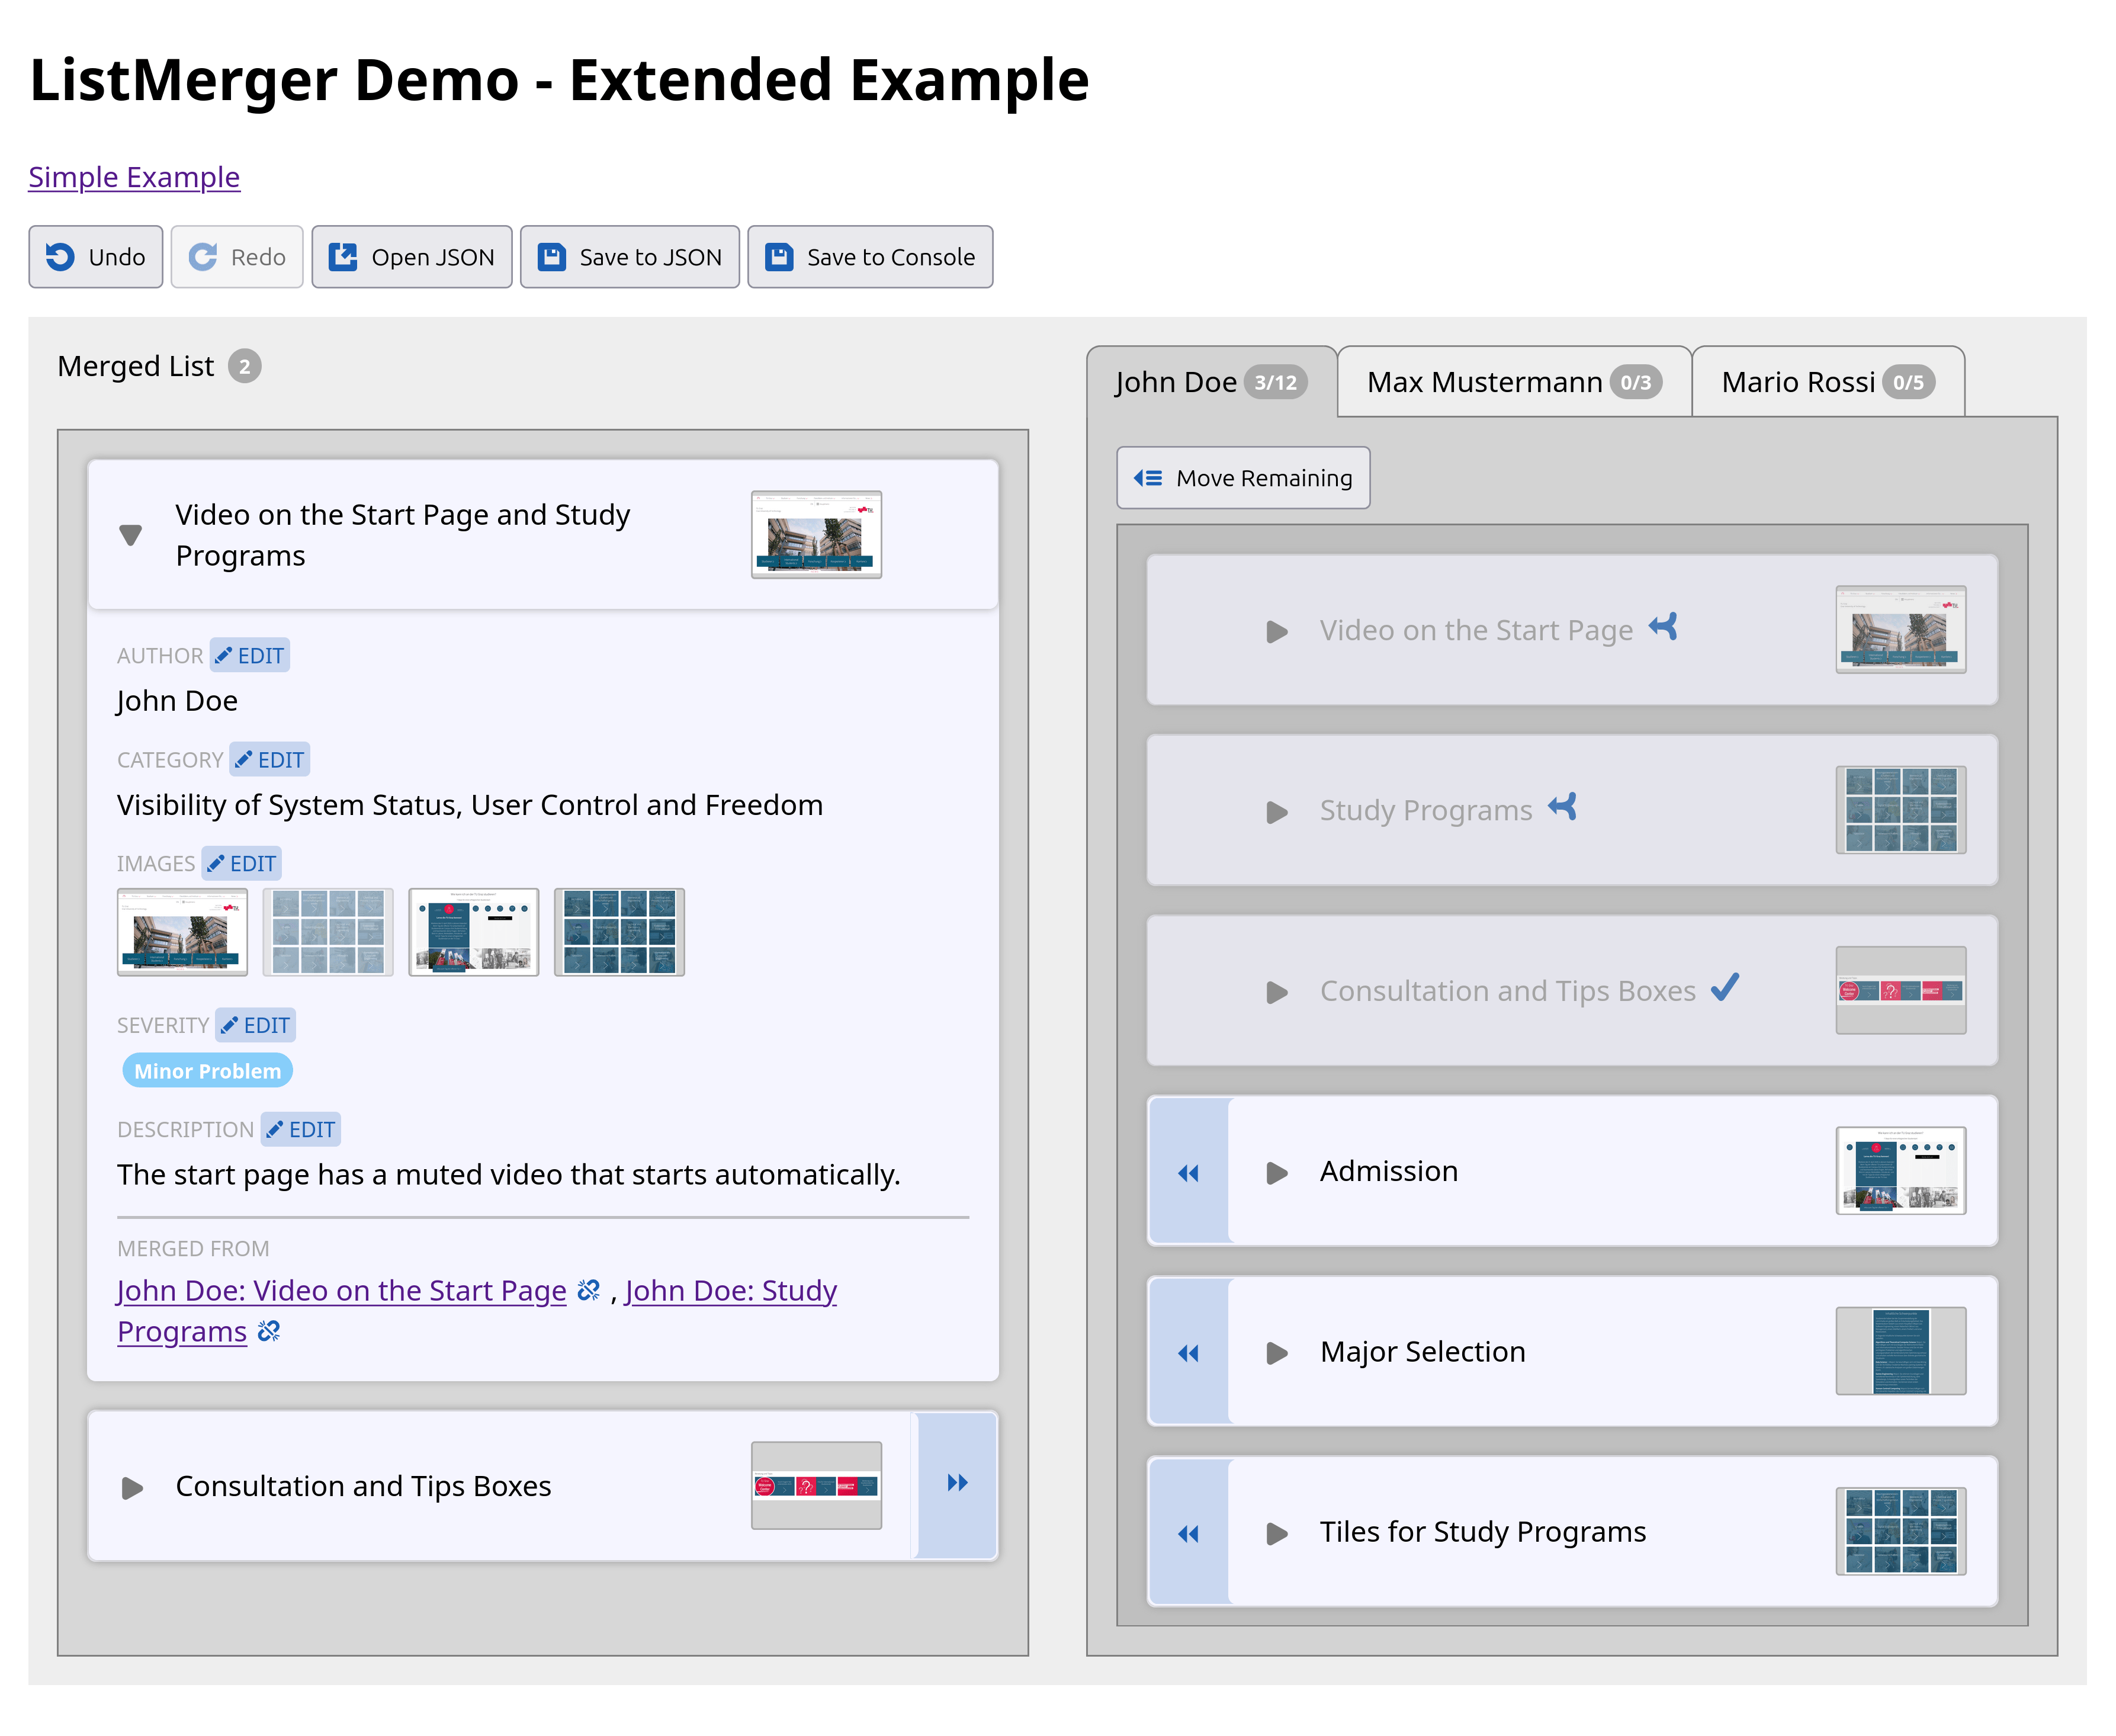
\includegraphics[frame,keepaspectratio,width=\linewidth,height=\halfh]
{images/full-i.png}
\caption[ListMerger Example]{%
An example implementation of ListMerger. Merged origin items (right top)
and moved origin items appear greyed out and annotated with a merge,
respectively moved icon. The merged item itself (left) contains links to
them. Items can be dragged and dropped from the right to the left.
\imgcredit{Screenshot by Martin Rabensteiner.}
}
\label{fig:enduser-overview}
\end{figure}

This chapter serves explanatory notes for end users of this library.
Note that some procedures and designs described in this chapter may
differ for the actual implementation in the specific tool. An example
implementation can be seen in Figure~\ref{fig:enduser-overview} and
explanations refer to this architecture.



\section{Functionality}
The main objective of this library is to have a number of lists, the
\emph{origin lists} on one side (usually right) and an aggregated list
on the other side (left), the \emph{mergelist}. Users can switch between
these origin lists via tabs, or on more narrow screens with a select
box. Items can be dragged and dropped from one list on the right to the
mergelist on the left. An item is inserted at the location where it is
dropped. The \uiname{Move Remaining} button can be used to move all
existing items of a list to the mergelist. The appearance of items in
the list, their extended view, and the merge dialogue are dependent on
the individual implementation.

By dragging one item over another in the mergelist, those items can be
merged. By dragging items in the mergelist around, they can be
rearranged. \uiname{Undo} and \uiname{Redo} let the user jump through
the history.

% Saving
The behaviour of saving is given by the individual implementation and
can automatically, or by clicking a \uiname{Save} button. Data is in
principle stored in the JSON format. When a saved file is opened again,
it must be noted that the file format has the same version as required
by the library.

% Indicators
Next to the tab titles can be small numbers to indicate the current
state of the list. For origin lists, they count how much of items have
been added or merged into the mergelist out of the total number per
list. For the mergelist, the indicator shows the total number of items
in the list, not necessarily how much have been added.

% Editing
Properties of items can be edited by clicking on them. Text-only
properties are then directly editable and saved as soon as the focus is
changed to another element by mouse or keyboard. More complex
properties, like select boxes, need a double click to change to editing
mode.


\section{Keyboard Shortcuts}
ListMerger offers shortcuts to ease the use with a keyboard. These
shortcuts are:
\begin{itemize}
    \item \liintro{Ctrl + Z}: Undo.
    \item \liintro{Ctrl + Y}: Redo.
    \item \liintro{C}: Collapse all \elname{details} elements.
    \item \liintro{M}: Move all remaining elements from an origin list
      to the mergelist.
    \item \liintro{[1-9]}: Switch the current tab of lists. The number
      indicates their index.
\end{itemize}

